% Created by tikzDevice version 0.12 on 2019-05-24 17:17:13
% !TEX encoding = UTF-8 Unicode
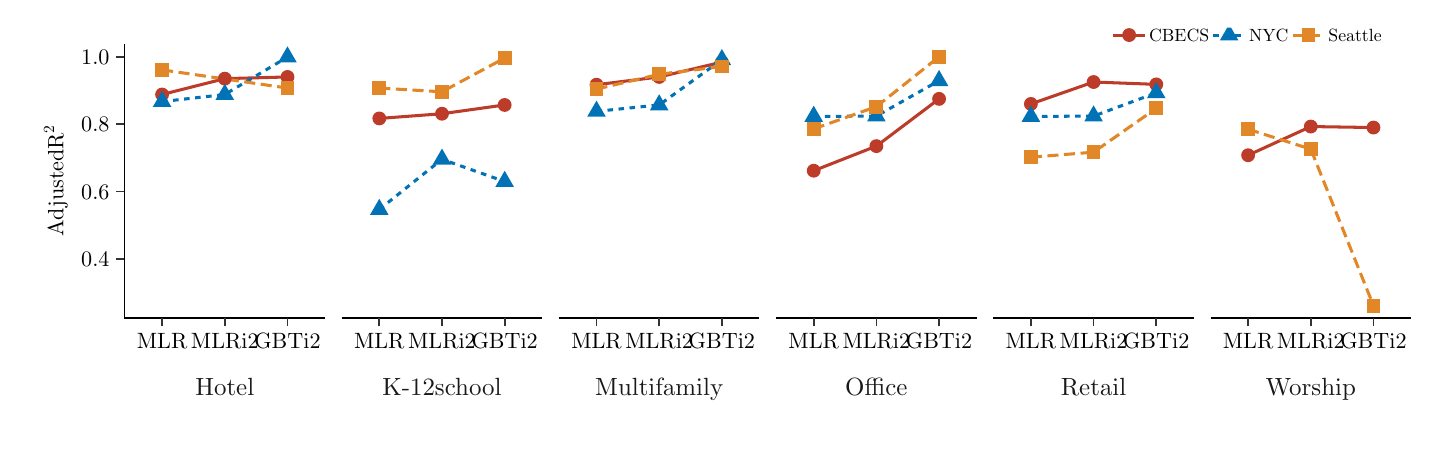
\begin{tikzpicture}[x=1pt,y=1pt]
\definecolor{fillColor}{RGB}{255,255,255}
\path[use as bounding box,fill=fillColor,fill opacity=0.00] (0,0) rectangle (505.89,144.54);
\begin{scope}
\path[clip] (  0.00,  0.00) rectangle (505.89,144.54);
\definecolor{drawColor}{RGB}{255,255,255}
\definecolor{fillColor}{RGB}{255,255,255}

\path[draw=drawColor,line width= 0.6pt,line join=round,line cap=round,fill=fillColor] (  0.00,  0.00) rectangle (505.89,144.54);
\end{scope}
\begin{scope}
\path[clip] ( 34.98, 39.60) rectangle (107.47,138.54);
\definecolor{fillColor}{RGB}{255,255,255}

\path[fill=fillColor] ( 34.98, 39.60) rectangle (107.47,138.54);
\definecolor{drawColor}{RGB}{188,60,41}

\path[draw=drawColor,line width= 1.1pt,line join=round] ( 48.57,120.39) --
	( 71.23,126.12) --
	( 93.88,126.73);
\definecolor{drawColor}{RGB}{0,114,181}

\path[draw=drawColor,line width= 1.1pt,dash pattern=on 2pt off 2pt ,line join=round] ( 48.57,117.83) --
	( 71.23,120.39) --
	( 93.88,133.92);
\definecolor{drawColor}{RGB}{225,135,39}

\path[draw=drawColor,line width= 1.1pt,dash pattern=on 4pt off 2pt ,line join=round] ( 48.57,129.29) --
	( 93.88,122.71);
\definecolor{fillColor}{RGB}{188,60,41}

\path[fill=fillColor] ( 48.57,120.39) circle (  2.50);

\path[fill=fillColor] ( 71.23,126.12) circle (  2.50);

\path[fill=fillColor] ( 93.88,126.73) circle (  2.50);
\definecolor{fillColor}{RGB}{0,114,181}

\path[fill=fillColor] ( 48.57,121.72) --
	( 51.94,115.89) --
	( 45.21,115.89) --
	cycle;

\path[fill=fillColor] ( 71.23,124.28) --
	( 74.59,118.45) --
	( 67.86,118.45) --
	cycle;

\path[fill=fillColor] ( 93.88,137.80) --
	( 97.24,131.98) --
	( 90.51,131.98) --
	cycle;
\definecolor{fillColor}{RGB}{225,135,39}

\path[fill=fillColor] ( 46.08,126.79) --
	( 51.07,126.79) --
	( 51.07,131.79) --
	( 46.08,131.79) --
	cycle;

\path[fill=fillColor] ( 91.38,120.21) --
	( 96.37,120.21) --
	( 96.37,125.21) --
	( 91.38,125.21) --
	cycle;
\end{scope}
\begin{scope}
\path[clip] (113.47, 39.60) rectangle (185.95,138.54);
\definecolor{fillColor}{RGB}{255,255,255}

\path[fill=fillColor] (113.47, 39.60) rectangle (185.95,138.54);
\definecolor{drawColor}{RGB}{188,60,41}

\path[draw=drawColor,line width= 1.1pt,line join=round] (127.06,111.74) --
	(149.71,113.44) --
	(172.36,116.61);
\definecolor{drawColor}{RGB}{0,114,181}

\path[draw=drawColor,line width= 1.1pt,dash pattern=on 2pt off 2pt ,line join=round] (127.06, 78.83) --
	(149.71, 96.99) --
	(172.36, 88.95);
\definecolor{drawColor}{RGB}{225,135,39}

\path[draw=drawColor,line width= 1.1pt,dash pattern=on 4pt off 2pt ,line join=round] (127.06,122.71) --
	(149.71,121.37) --
	(172.36,133.56);
\definecolor{fillColor}{RGB}{188,60,41}

\path[fill=fillColor] (127.06,111.74) circle (  2.50);

\path[fill=fillColor] (149.71,113.44) circle (  2.50);

\path[fill=fillColor] (172.36,116.61) circle (  2.50);
\definecolor{fillColor}{RGB}{0,114,181}

\path[fill=fillColor] (127.06, 82.71) --
	(130.42, 76.89) --
	(123.69, 76.89) --
	cycle;

\path[fill=fillColor] (149.71,100.87) --
	(153.07, 95.05) --
	(146.35, 95.05) --
	cycle;

\path[fill=fillColor] (172.36, 92.83) --
	(175.72, 87.00) --
	(169.00, 87.00) --
	cycle;
\definecolor{fillColor}{RGB}{225,135,39}

\path[fill=fillColor] (124.56,120.21) --
	(129.56,120.21) --
	(129.56,125.21) --
	(124.56,125.21) --
	cycle;

\path[fill=fillColor] (147.21,118.87) --
	(152.21,118.87) --
	(152.21,123.86) --
	(147.21,123.86) --
	cycle;

\path[fill=fillColor] (169.86,131.06) --
	(174.86,131.06) --
	(174.86,136.05) --
	(169.86,136.05) --
	cycle;
\end{scope}
\begin{scope}
\path[clip] (191.95, 39.60) rectangle (264.44,138.54);
\definecolor{fillColor}{RGB}{255,255,255}

\path[fill=fillColor] (191.95, 39.60) rectangle (264.44,138.54);
\definecolor{drawColor}{RGB}{188,60,41}

\path[draw=drawColor,line width= 1.1pt,line join=round] (205.54,123.93) --
	(228.19,126.73) --
	(250.85,132.09);
\definecolor{drawColor}{RGB}{0,114,181}

\path[draw=drawColor,line width= 1.1pt,dash pattern=on 2pt off 2pt ,line join=round] (205.54,114.30) --
	(228.19,116.61) --
	(250.85,132.95);
\definecolor{drawColor}{RGB}{225,135,39}

\path[draw=drawColor,line width= 1.1pt,dash pattern=on 4pt off 2pt ,line join=round] (205.54,122.34) --
	(228.19,127.70) --
	(250.85,130.51);
\definecolor{fillColor}{RGB}{188,60,41}

\path[fill=fillColor] (205.54,123.93) circle (  2.50);

\path[fill=fillColor] (228.19,126.73) circle (  2.50);

\path[fill=fillColor] (250.85,132.09) circle (  2.50);
\definecolor{fillColor}{RGB}{0,114,181}

\path[fill=fillColor] (205.54,118.18) --
	(208.91,112.36) --
	(202.18,112.36) --
	cycle;

\path[fill=fillColor] (228.19,120.50) --
	(231.56,114.67) --
	(224.83,114.67) --
	cycle;

\path[fill=fillColor] (250.85,136.83) --
	(254.21,131.00) --
	(247.48,131.00) --
	cycle;
\definecolor{fillColor}{RGB}{225,135,39}

\path[fill=fillColor] (203.05,119.84) --
	(208.04,119.84) --
	(208.04,124.84) --
	(203.05,124.84) --
	cycle;

\path[fill=fillColor] (225.70,125.21) --
	(230.69,125.21) --
	(230.69,130.20) --
	(225.70,130.20) --
	cycle;

\path[fill=fillColor] (248.35,128.01) --
	(253.34,128.01) --
	(253.34,133.01) --
	(248.35,133.01) --
	cycle;
\end{scope}
\begin{scope}
\path[clip] (270.44, 39.60) rectangle (342.92,138.54);
\definecolor{fillColor}{RGB}{255,255,255}

\path[fill=fillColor] (270.44, 39.60) rectangle (342.92,138.54);
\definecolor{drawColor}{RGB}{188,60,41}

\path[draw=drawColor,line width= 1.1pt,line join=round] (284.03, 92.85) --
	(306.68,101.74) --
	(329.33,118.81);
\definecolor{drawColor}{RGB}{0,114,181}

\path[draw=drawColor,line width= 1.1pt,dash pattern=on 2pt off 2pt ,line join=round] (284.03,112.47) --
	(306.68,112.59) --
	(329.33,125.39);
\definecolor{drawColor}{RGB}{225,135,39}

\path[draw=drawColor,line width= 1.1pt,dash pattern=on 4pt off 2pt ,line join=round] (284.03,107.96) --
	(306.68,116.00) --
	(329.33,134.04);
\definecolor{fillColor}{RGB}{188,60,41}

\path[fill=fillColor] (284.03, 92.85) circle (  2.50);

\path[fill=fillColor] (306.68,101.74) circle (  2.50);

\path[fill=fillColor] (329.33,118.81) circle (  2.50);
\definecolor{fillColor}{RGB}{0,114,181}

\path[fill=fillColor] (284.03,116.35) --
	(287.39,110.53) --
	(280.66,110.53) --
	cycle;

\path[fill=fillColor] (306.68,116.48) --
	(310.04,110.65) --
	(303.31,110.65) --
	cycle;

\path[fill=fillColor] (329.33,129.27) --
	(332.69,123.45) --
	(325.97,123.45) --
	cycle;
\definecolor{fillColor}{RGB}{225,135,39}

\path[fill=fillColor] (281.53,105.46) --
	(286.52,105.46) --
	(286.52,110.46) --
	(281.53,110.46) --
	cycle;

\path[fill=fillColor] (304.18,113.51) --
	(309.18,113.51) --
	(309.18,118.50) --
	(304.18,118.50) --
	cycle;

\path[fill=fillColor] (326.83,131.54) --
	(331.83,131.54) --
	(331.83,136.54) --
	(326.83,136.54) --
	cycle;
\end{scope}
\begin{scope}
\path[clip] (348.92, 39.60) rectangle (421.41,138.54);
\definecolor{fillColor}{RGB}{255,255,255}

\path[fill=fillColor] (348.92, 39.60) rectangle (421.41,138.54);
\definecolor{drawColor}{RGB}{188,60,41}

\path[draw=drawColor,line width= 1.1pt,line join=round] (362.51,116.98) --
	(385.16,124.90) --
	(407.81,124.05);
\definecolor{drawColor}{RGB}{0,114,181}

\path[draw=drawColor,line width= 1.1pt,dash pattern=on 2pt off 2pt ,line join=round] (362.51,112.47) --
	(385.16,112.59) --
	(407.81,121.00);
\definecolor{drawColor}{RGB}{225,135,39}

\path[draw=drawColor,line width= 1.1pt,dash pattern=on 4pt off 2pt ,line join=round] (362.51, 97.72) --
	(385.16, 99.55) --
	(407.81,115.39);
\definecolor{fillColor}{RGB}{188,60,41}

\path[fill=fillColor] (362.51,116.98) circle (  2.50);

\path[fill=fillColor] (385.16,124.90) circle (  2.50);

\path[fill=fillColor] (407.81,124.05) circle (  2.50);
\definecolor{fillColor}{RGB}{0,114,181}

\path[fill=fillColor] (362.51,116.35) --
	(365.88,110.53) --
	(359.15,110.53) --
	cycle;

\path[fill=fillColor] (385.16,116.48) --
	(388.53,110.65) --
	(381.80,110.65) --
	cycle;

\path[fill=fillColor] (407.81,124.89) --
	(411.18,119.06) --
	(404.45,119.06) --
	cycle;
\definecolor{fillColor}{RGB}{225,135,39}

\path[fill=fillColor] (360.01, 95.22) --
	(365.01, 95.22) --
	(365.01,100.22) --
	(360.01,100.22) --
	cycle;

\path[fill=fillColor] (382.67, 97.05) --
	(387.66, 97.05) --
	(387.66,102.05) --
	(382.67,102.05) --
	cycle;

\path[fill=fillColor] (405.32,112.90) --
	(410.31,112.90) --
	(410.31,117.89) --
	(405.32,117.89) --
	cycle;
\end{scope}
\begin{scope}
\path[clip] (427.41, 39.60) rectangle (499.89,138.54);
\definecolor{fillColor}{RGB}{255,255,255}

\path[fill=fillColor] (427.41, 39.60) rectangle (499.89,138.54);
\definecolor{drawColor}{RGB}{188,60,41}

\path[draw=drawColor,line width= 1.1pt,line join=round] (441.00, 98.45) --
	(463.65,108.81) --
	(486.30,108.45);
\definecolor{drawColor}{RGB}{225,135,39}

\path[draw=drawColor,line width= 1.1pt,dash pattern=on 4pt off 2pt ,line join=round] (441.00,107.84) --
	(463.65,100.65) --
	(486.30, 44.09);
\definecolor{fillColor}{RGB}{188,60,41}

\path[fill=fillColor] (441.00, 98.45) circle (  2.50);

\path[fill=fillColor] (463.65,108.81) circle (  2.50);

\path[fill=fillColor] (486.30,108.45) circle (  2.50);
\definecolor{fillColor}{RGB}{225,135,39}

\path[fill=fillColor] (438.50,105.34) --
	(443.49,105.34) --
	(443.49,110.34) --
	(438.50,110.34) --
	cycle;

\path[fill=fillColor] (461.15, 98.15) --
	(466.15, 98.15) --
	(466.15,103.14) --
	(461.15,103.14) --
	cycle;

\path[fill=fillColor] (483.80, 41.60) --
	(488.80, 41.60) --
	(488.80, 46.59) --
	(483.80, 46.59) --
	cycle;
\end{scope}
\begin{scope}
\path[clip] ( 34.98,  6.00) rectangle (107.47, 23.74);
\definecolor{drawColor}{gray}{0.10}

\node[text=drawColor,anchor=base,inner sep=0pt, outer sep=0pt, scale=  0.90] at ( 71.23, 11.77) {Hotel};
\end{scope}
\begin{scope}
\path[clip] (113.47,  6.00) rectangle (185.95, 23.74);
\definecolor{drawColor}{gray}{0.10}

\node[text=drawColor,anchor=base,inner sep=0pt, outer sep=0pt, scale=  0.90] at (149.71, 11.77) {K-12school};
\end{scope}
\begin{scope}
\path[clip] (191.95,  6.00) rectangle (264.44, 23.74);
\definecolor{drawColor}{gray}{0.10}

\node[text=drawColor,anchor=base,inner sep=0pt, outer sep=0pt, scale=  0.90] at (228.19, 11.77) {Multifamily};
\end{scope}
\begin{scope}
\path[clip] (270.44,  6.00) rectangle (342.92, 23.74);
\definecolor{drawColor}{gray}{0.10}

\node[text=drawColor,anchor=base,inner sep=0pt, outer sep=0pt, scale=  0.90] at (306.68, 11.77) {Office};
\end{scope}
\begin{scope}
\path[clip] (348.92,  6.00) rectangle (421.41, 23.74);
\definecolor{drawColor}{gray}{0.10}

\node[text=drawColor,anchor=base,inner sep=0pt, outer sep=0pt, scale=  0.90] at (385.16, 11.77) {Retail};
\end{scope}
\begin{scope}
\path[clip] (427.41,  6.00) rectangle (499.89, 23.74);
\definecolor{drawColor}{gray}{0.10}

\node[text=drawColor,anchor=base,inner sep=0pt, outer sep=0pt, scale=  0.90] at (463.65, 11.77) {Worship};
\end{scope}
\begin{scope}
\path[clip] (  0.00,  0.00) rectangle (505.89,144.54);
\definecolor{drawColor}{RGB}{0,0,0}

\path[draw=drawColor,line width= 0.6pt,line join=round] ( 34.98, 39.60) --
	(107.47, 39.60);
\end{scope}
\begin{scope}
\path[clip] (  0.00,  0.00) rectangle (505.89,144.54);
\definecolor{drawColor}{gray}{0.20}

\path[draw=drawColor,line width= 0.6pt,line join=round] ( 48.57, 36.60) --
	( 48.57, 39.60);

\path[draw=drawColor,line width= 0.6pt,line join=round] ( 71.23, 36.60) --
	( 71.23, 39.60);

\path[draw=drawColor,line width= 0.6pt,line join=round] ( 93.88, 36.60) --
	( 93.88, 39.60);
\end{scope}
\begin{scope}
\path[clip] (  0.00,  0.00) rectangle (505.89,144.54);
\definecolor{drawColor}{RGB}{0,0,0}

\node[text=drawColor,anchor=base,inner sep=0pt, outer sep=0pt, scale=  0.80] at ( 48.57, 28.69) {MLR};

\node[text=drawColor,anchor=base,inner sep=0pt, outer sep=0pt, scale=  0.80] at ( 71.23, 28.69) {MLRi2};

\node[text=drawColor,anchor=base,inner sep=0pt, outer sep=0pt, scale=  0.80] at ( 93.88, 28.69) {GBTi2};
\end{scope}
\begin{scope}
\path[clip] (  0.00,  0.00) rectangle (505.89,144.54);
\definecolor{drawColor}{RGB}{0,0,0}

\path[draw=drawColor,line width= 0.6pt,line join=round] (113.47, 39.60) --
	(185.95, 39.60);
\end{scope}
\begin{scope}
\path[clip] (  0.00,  0.00) rectangle (505.89,144.54);
\definecolor{drawColor}{gray}{0.20}

\path[draw=drawColor,line width= 0.6pt,line join=round] (127.06, 36.60) --
	(127.06, 39.60);

\path[draw=drawColor,line width= 0.6pt,line join=round] (149.71, 36.60) --
	(149.71, 39.60);

\path[draw=drawColor,line width= 0.6pt,line join=round] (172.36, 36.60) --
	(172.36, 39.60);
\end{scope}
\begin{scope}
\path[clip] (  0.00,  0.00) rectangle (505.89,144.54);
\definecolor{drawColor}{RGB}{0,0,0}

\node[text=drawColor,anchor=base,inner sep=0pt, outer sep=0pt, scale=  0.80] at (127.06, 28.69) {MLR};

\node[text=drawColor,anchor=base,inner sep=0pt, outer sep=0pt, scale=  0.80] at (149.71, 28.69) {MLRi2};

\node[text=drawColor,anchor=base,inner sep=0pt, outer sep=0pt, scale=  0.80] at (172.36, 28.69) {GBTi2};
\end{scope}
\begin{scope}
\path[clip] (  0.00,  0.00) rectangle (505.89,144.54);
\definecolor{drawColor}{RGB}{0,0,0}

\path[draw=drawColor,line width= 0.6pt,line join=round] (191.95, 39.60) --
	(264.44, 39.60);
\end{scope}
\begin{scope}
\path[clip] (  0.00,  0.00) rectangle (505.89,144.54);
\definecolor{drawColor}{gray}{0.20}

\path[draw=drawColor,line width= 0.6pt,line join=round] (205.54, 36.60) --
	(205.54, 39.60);

\path[draw=drawColor,line width= 0.6pt,line join=round] (228.19, 36.60) --
	(228.19, 39.60);

\path[draw=drawColor,line width= 0.6pt,line join=round] (250.85, 36.60) --
	(250.85, 39.60);
\end{scope}
\begin{scope}
\path[clip] (  0.00,  0.00) rectangle (505.89,144.54);
\definecolor{drawColor}{RGB}{0,0,0}

\node[text=drawColor,anchor=base,inner sep=0pt, outer sep=0pt, scale=  0.80] at (205.54, 28.69) {MLR};

\node[text=drawColor,anchor=base,inner sep=0pt, outer sep=0pt, scale=  0.80] at (228.19, 28.69) {MLRi2};

\node[text=drawColor,anchor=base,inner sep=0pt, outer sep=0pt, scale=  0.80] at (250.85, 28.69) {GBTi2};
\end{scope}
\begin{scope}
\path[clip] (  0.00,  0.00) rectangle (505.89,144.54);
\definecolor{drawColor}{RGB}{0,0,0}

\path[draw=drawColor,line width= 0.6pt,line join=round] (270.44, 39.60) --
	(342.92, 39.60);
\end{scope}
\begin{scope}
\path[clip] (  0.00,  0.00) rectangle (505.89,144.54);
\definecolor{drawColor}{gray}{0.20}

\path[draw=drawColor,line width= 0.6pt,line join=round] (284.03, 36.60) --
	(284.03, 39.60);

\path[draw=drawColor,line width= 0.6pt,line join=round] (306.68, 36.60) --
	(306.68, 39.60);

\path[draw=drawColor,line width= 0.6pt,line join=round] (329.33, 36.60) --
	(329.33, 39.60);
\end{scope}
\begin{scope}
\path[clip] (  0.00,  0.00) rectangle (505.89,144.54);
\definecolor{drawColor}{RGB}{0,0,0}

\node[text=drawColor,anchor=base,inner sep=0pt, outer sep=0pt, scale=  0.80] at (284.03, 28.69) {MLR};

\node[text=drawColor,anchor=base,inner sep=0pt, outer sep=0pt, scale=  0.80] at (306.68, 28.69) {MLRi2};

\node[text=drawColor,anchor=base,inner sep=0pt, outer sep=0pt, scale=  0.80] at (329.33, 28.69) {GBTi2};
\end{scope}
\begin{scope}
\path[clip] (  0.00,  0.00) rectangle (505.89,144.54);
\definecolor{drawColor}{RGB}{0,0,0}

\path[draw=drawColor,line width= 0.6pt,line join=round] (348.92, 39.60) --
	(421.41, 39.60);
\end{scope}
\begin{scope}
\path[clip] (  0.00,  0.00) rectangle (505.89,144.54);
\definecolor{drawColor}{gray}{0.20}

\path[draw=drawColor,line width= 0.6pt,line join=round] (362.51, 36.60) --
	(362.51, 39.60);

\path[draw=drawColor,line width= 0.6pt,line join=round] (385.16, 36.60) --
	(385.16, 39.60);

\path[draw=drawColor,line width= 0.6pt,line join=round] (407.81, 36.60) --
	(407.81, 39.60);
\end{scope}
\begin{scope}
\path[clip] (  0.00,  0.00) rectangle (505.89,144.54);
\definecolor{drawColor}{RGB}{0,0,0}

\node[text=drawColor,anchor=base,inner sep=0pt, outer sep=0pt, scale=  0.80] at (362.51, 28.69) {MLR};

\node[text=drawColor,anchor=base,inner sep=0pt, outer sep=0pt, scale=  0.80] at (385.16, 28.69) {MLRi2};

\node[text=drawColor,anchor=base,inner sep=0pt, outer sep=0pt, scale=  0.80] at (407.81, 28.69) {GBTi2};
\end{scope}
\begin{scope}
\path[clip] (  0.00,  0.00) rectangle (505.89,144.54);
\definecolor{drawColor}{RGB}{0,0,0}

\path[draw=drawColor,line width= 0.6pt,line join=round] (427.41, 39.60) --
	(499.89, 39.60);
\end{scope}
\begin{scope}
\path[clip] (  0.00,  0.00) rectangle (505.89,144.54);
\definecolor{drawColor}{gray}{0.20}

\path[draw=drawColor,line width= 0.6pt,line join=round] (441.00, 36.60) --
	(441.00, 39.60);

\path[draw=drawColor,line width= 0.6pt,line join=round] (463.65, 36.60) --
	(463.65, 39.60);

\path[draw=drawColor,line width= 0.6pt,line join=round] (486.30, 36.60) --
	(486.30, 39.60);
\end{scope}
\begin{scope}
\path[clip] (  0.00,  0.00) rectangle (505.89,144.54);
\definecolor{drawColor}{RGB}{0,0,0}

\node[text=drawColor,anchor=base,inner sep=0pt, outer sep=0pt, scale=  0.80] at (441.00, 28.69) {MLR};

\node[text=drawColor,anchor=base,inner sep=0pt, outer sep=0pt, scale=  0.80] at (463.65, 28.69) {MLRi2};

\node[text=drawColor,anchor=base,inner sep=0pt, outer sep=0pt, scale=  0.80] at (486.30, 28.69) {GBTi2};
\end{scope}
\begin{scope}
\path[clip] (  0.00,  0.00) rectangle (505.89,144.54);
\definecolor{drawColor}{RGB}{0,0,0}

\path[draw=drawColor,line width= 0.6pt,line join=round] ( 34.98, 39.60) --
	( 34.98,138.54);
\end{scope}
\begin{scope}
\path[clip] (  0.00,  0.00) rectangle (505.89,144.54);
\definecolor{drawColor}{RGB}{0,0,0}

\node[text=drawColor,anchor=base east,inner sep=0pt, outer sep=0pt, scale=  0.80] at ( 29.58, 58.16) {0.4};

\node[text=drawColor,anchor=base east,inner sep=0pt, outer sep=0pt, scale=  0.80] at ( 29.58, 82.53) {0.6};

\node[text=drawColor,anchor=base east,inner sep=0pt, outer sep=0pt, scale=  0.80] at ( 29.58,106.91) {0.8};

\node[text=drawColor,anchor=base east,inner sep=0pt, outer sep=0pt, scale=  0.80] at ( 29.58,131.29) {1.0};
\end{scope}
\begin{scope}
\path[clip] (  0.00,  0.00) rectangle (505.89,144.54);
\definecolor{drawColor}{gray}{0.20}

\path[draw=drawColor,line width= 0.6pt,line join=round] ( 31.98, 60.91) --
	( 34.98, 60.91);

\path[draw=drawColor,line width= 0.6pt,line join=round] ( 31.98, 85.29) --
	( 34.98, 85.29);

\path[draw=drawColor,line width= 0.6pt,line join=round] ( 31.98,109.67) --
	( 34.98,109.67);

\path[draw=drawColor,line width= 0.6pt,line join=round] ( 31.98,134.04) --
	( 34.98,134.04);
\end{scope}
\begin{scope}
\path[clip] (  0.00,  0.00) rectangle (505.89,144.54);
\definecolor{drawColor}{RGB}{0,0,0}

\node[text=drawColor,rotate= 90.00,anchor=base west,inner sep=0pt, outer sep=0pt, scale=  0.80] at ( 12.86, 69.04) {Adjusted };

\node[text=drawColor,rotate= 90.00,anchor=base west,inner sep=0pt, outer sep=0pt, scale=  0.80] at ( 12.86,100.41) {R};

\node[text=drawColor,rotate= 90.00,anchor=base west,inner sep=0pt, outer sep=0pt, scale=  0.56] at (  9.59,106.30) {2};
\end{scope}
\begin{scope}
\path[clip] (  0.00,  0.00) rectangle (505.89,144.54);
\definecolor{fillColor}{RGB}{255,255,255}

\path[fill=fillColor] (384.78,128.65) rectangle (495.24,155.10);
\end{scope}
\begin{scope}
\path[clip] (  0.00,  0.00) rectangle (505.89,144.54);
\definecolor{drawColor}{RGB}{188,60,41}

\path[draw=drawColor,line width= 1.1pt,line join=round] (392.23,141.87) -- (403.79,141.87);
\end{scope}
\begin{scope}
\path[clip] (  0.00,  0.00) rectangle (505.89,144.54);
\definecolor{fillColor}{RGB}{188,60,41}

\path[fill=fillColor] (398.01,141.87) circle (  2.50);
\end{scope}
\begin{scope}
\path[clip] (  0.00,  0.00) rectangle (505.89,144.54);
\definecolor{drawColor}{RGB}{0,114,181}

\path[draw=drawColor,line width= 1.1pt,dash pattern=on 2pt off 2pt ,line join=round] (428.36,141.87) -- (439.93,141.87);
\end{scope}
\begin{scope}
\path[clip] (  0.00,  0.00) rectangle (505.89,144.54);
\definecolor{fillColor}{RGB}{0,114,181}

\path[fill=fillColor] (434.85,144.54) --
	(437.51,139.93) --
	(430.78,139.93) --
	(433.44,144.54) --
	cycle;
\end{scope}
\begin{scope}
\path[clip] (  0.00,  0.00) rectangle (505.89,144.54);
\definecolor{drawColor}{RGB}{225,135,39}

\path[draw=drawColor,line width= 1.1pt,dash pattern=on 4pt off 2pt ,line join=round] (457.04,141.87) -- (468.60,141.87);
\end{scope}
\begin{scope}
\path[clip] (  0.00,  0.00) rectangle (505.89,144.54);
\definecolor{fillColor}{RGB}{225,135,39}

\path[fill=fillColor] (460.32,139.37) --
	(465.32,139.37) --
	(465.32,144.37) --
	(460.32,144.37) --
	cycle;
\end{scope}
\begin{scope}
\path[clip] (  0.00,  0.00) rectangle (505.89,144.54);
\definecolor{drawColor}{RGB}{0,0,0}

\node[text=drawColor,anchor=base west,inner sep=0pt, outer sep=0pt, scale=  0.64] at (405.24,139.67) {CBECS};
\end{scope}
\begin{scope}
\path[clip] (  0.00,  0.00) rectangle (505.89,144.54);
\definecolor{drawColor}{RGB}{0,0,0}

\node[text=drawColor,anchor=base west,inner sep=0pt, outer sep=0pt, scale=  0.64] at (441.37,139.67) {NYC};
\end{scope}
\begin{scope}
\path[clip] (  0.00,  0.00) rectangle (505.89,144.54);
\definecolor{drawColor}{RGB}{0,0,0}

\node[text=drawColor,anchor=base west,inner sep=0pt, outer sep=0pt, scale=  0.64] at (470.05,139.67) {Seattle};
\end{scope}
\end{tikzpicture}
